\subsection{Using the Python Plugin}

Writing plugins in Python is much simpler than using C++. To create a PyQGIS
plugin, you need QGIS 0.9, Python, PyQt, and the Qt developer tools 
\cite{sherman07}.

When QGIS starts up it scans certain directories looking for both C++ and
Python plugins. For a file (shared library, DLL, or python script) to be
recognized as a plugin it has to have a specific signature. For Python scripts
it's pretty simple. QGIS looks in the following locations under the
installation directory:

\begin{itemize}
\item \textbf{Linux and other Unix}: ./share/qgis/python/plugins
\item \textbf{Mac OS X}: ./Contents/MacOS/share/qgis/python/plugins
\item \textbf{Windows}: .\textbackslash share\textbackslash QGIS\textbackslash
python\textbackslash plugins
\end{itemize}

Each Python plugin is contained in its own directory. When QGIS starts up it will
scan each subdirectory in \textsl{share/qgis/python/plugins} and initialize
any plugins it finds. Once that's done, the plugin will show up in the plugin
manager.  

Let's create a plugin to fill a gap in the QGIS interface. This plugin will
allow us to create a new PostGIS layer for us to digitize. It will be a
simple plugin and pretty rough, but it illustrates how to get started
writing your own PyQGIS plugins.

\subsubsection{Setting up the Structure}
The first thing we need to do is set up the structure for our plugin. In
this example we'll be developing our plugin on Linux but the method is
the same, just adapt some of the file system commands as appropriate for
your platform. QGIS is installed in a directory named
\textsl{qgis\_09} in our home directory. Let's create the directory for 
the plugin.

\begin{verbatim}
mkdir ~/qgis_09/share/qgis/python/plugins/new_layer
\end{verbatim}

To get started, we need to create the following files in the \textsl{new\_layer} directory
  (we'll need some additional files in a bit):

\begin{verbatim}
__init__.py 
resources.py
resources.qrc
newlayer.py
\end{verbatim} 

\subsubsection{Making the Plugin Recognizable}

Initializing the plugin is done in the \textsl{\_\_init\_\_.py} script. For our 
\textsl{NewLayer} plugin the script contains:

\begin{verbatim}
1 # load NewLayer class from file newlayer.py
2 from newlayer import NewLayer
3 def name():
4   return "New PostGIS layer"
5 def description():
6   return "Creates a new empty Postgis layer"
7 def version():
8   return "Version 0.1"
9 def classFactory(iface):
10   return NewLayer(iface)
\end{verbatim} 

The mandatory things a plugin must return are a name, description, and
version, all of which are implemented in our script above. Each method
simply returns a string with the appropriate information. The other
requirement is the \textsl{classFactory} method that must
return a reference to the plugin itself (line 10), after 
receiving the \textbf{iface} object as an argument. With this simple code, 
QGIS will recognize our script as a plugin.

\subsubsection{Resources}

In order to have a nice icon for our plugin, we need a resources file
which we'll name \textsl{resources.qrc}. This is just a simple XML 
file that defines the icon resource:

\begin{verbatim}
 <RCC>
    <qresource prefix="/plugins/newlayer">
        <file>icon.png</file>
    </qresource>
</RCC> 
\end{verbatim} 

The resource file uses a prefix to prevent naming clashes with other
plugins - using the name of the plugin is usually sufficient.
The \textsl{icon.png} file is is just a PNG image that will be used 
in the toolbar when the plugin is activated. You can use any image, 
as long as it's 22x22 pixels (so it fits on the toolbar).

To turn the resource file into something the plugin can use, it must be 
compiled using the PyQt resource compiler:

\begin{verbatim}
  pyrcc4 -o resources.py resources.qrc
\end{verbatim}

The \textsl{-o} switch is used to specify the output file. Now that we 
have resources, we need a way to collect the information needed for creating 
a new layer.

\subsubsection{Creating the GUI}

Normally we would use the same tool that C++ developers use to create a 
GUI: Qt Designer. This is a visual design tool that allows you to create 
dialog and main windows by dragging and dropping widgets and defining 
their properties.

To design our NewLayer plugin we could get quite fancy and include widgets 
for field types and other options. However, since our time is limited, we'll 
use another means to collect the information we need to create the table. 
This will illustrate the concepts and then you can venture further using the 
tutorials on the QGIS blog.

To collect the user input, we'll use the \textsl{QInputDialog} class from
the Qt library.  This prompts the user for a single line of input. While it
will make our plugin a little crude, it serves to illustrate the concepts.

All we need to write now is the Python code to collect the input and create 
the table.

\subsubsection{Creating the Plugin}

Now that we have the preliminaries out of the way, we can get down to writing
the code that does the actual work.  Let's start by looking at the things we
need to import and the initialization of the plugin in \textsl{newlayer.py}.
 
\begin{verbatim}
1 # Import the PyQt and QGIS libraries
2 from PyQt4.QtCore import *
3 from PyQt4.QtGui import *
4 from qgis.core import *
5 import psycopg
6 # Initialize Qt resources from file resources.py
7 import resources
8
9 # Our main class for the plugin
10 class NewLayer:
11
12  def __init__(self, iface):
13    # Save reference to the QGIS interface
14    self.iface = iface
15
16  def initGui(self):
17    # Create action that will start plugin configuration
18    self.action = QAction(QIcon(":/plugins/newlayer/icon.png"),\
19      "New PosGIS Layer", self.iface.getMainWindow())
20    QObject.connect(self.action, SIGNAL("activated()"), self.run)
21
22    # Add toolbar button and menu item
23    self.iface.addToolBarIcon(self.action)
24    self.iface.addPluginMenu("&New PostGIS Layer...", self.action)
25
26  def unload(self):
27    # Remove the plugin menu item and icon
28    self.iface.removePluginMenu("&New PostGIS Layer...",self.action)
29    self.iface.removeToolBarIcon(self.action)
\end{verbatim}

In lines 2 through 7 we import the libraries needed for the plugin. 
This includes the PyQt libraries, the QGIS core library, and the Python 
PostgreSQL library psycopg. Every Python script that uses the QGIS 
libraries and PyQt needs to import the QtCore and QtGui libraries, as 
well as the QGIS core library.
This gives us access to the PyQt wrappers for our Qt objects (like our
input dialog) and the QGIS core libraries.  We also need to import the
\textsl{resources.py} file we created with the icon definition.

In line 10 we declare the class \textbf{NewLayer}. In the \textsl{\_\_init\_\_} 
method (lines 12 through 14) our class is initialized and passed the 
\textbf{iface} object from QGIS via the \textsl{classFactory} method
in line 10 of \_\_init\_\_.py. We store \textbf{iface} as a 
member variable so we can use it later. 

In lines 16 through 24 we initialize the GUI
elements for the plugin. In Qt, a \textbf{QAction} is used to create a
user interface action that can be used to create both a menu and toolbar
item. In our plugin, we use it for both. In line 18 we create the
action using our icon resource (note the prefix we specified in
\textsl{resources.qrc}). We also provide some text that will appear when
it is used in a menu or during a mouseover, and lastly we need to specify
the ``parent''. In a plugin, the parent is the main window of QGIS. The
\textbf{iface} object that we stored during initialization allows us to
get the reference to the main window in line 19.

Once the action is created, we can add it to both the toolbar and the
\textsl{Plugins} menu (lines 23 and 24).
That takes care of initializing the GUI for the plugin. The other thing we 
need to do is clean up after ourself when the plugin is unloaded. The 
\textsl{unload} method takes care of this by removing
the menu item and the tool from the toolbar (lines 28 and 29).

This takes care of the initialization stuff and getting our plugin to load
and unload nicely. Now let's look at the code that does the actual work.
It's all contained in the \textsl{run} method.

\begin{verbatim}
30 def run(self): 
31   # Get the user input, starting with the table name
32   table_name = QInputDialog.getText(None, "Table Name?", \
33     "Name for new PostGIS layer")
34   if table_name[0].length() > 0:
35     # Get the field names and types
36     fields = QInputDialog.getText(None, "Field Names", \
37      "Fields (separate with a comma)")
38     parts = fields[0].split(',')
39     # Create the SQL statement
40     sql = "create table " + table_name[0] + " (id int4 primary key, "
41     for fld in parts:
42      sql += fld + " varchar(10), "
43     sql = sql[0:-2]
44     sql += ")"
45     # Connect to the database
46     # First get the DSN
47     dsn = QInputDialog.getText(None, "Database DSN", \
48      "Enter the DSN for connecting to the database (dbname=db user=user)")
49     if dsn[0].length() > 0:
50      con = psycopg.connect(str(dsn[0]))
51      curs = con.cursor()
52      curs.execute(str(sql))
53      con.commit()
54      # add the geometry column
55      curs.execute("select AddGeometryColumn('" + str(table_name[0]) + \
56        "', 'the_geom', 4326, 'POLYGON', 2)")
57      con.commit()
58      # create the GIST index
59      curs.execute("create index sidx_" + str(table_name[0]) + " on " + \
60        str(table_name[0]) + " USING GIST(the_geom GIST_GEOMETRY_OPS)")
61        con.commit()
\end{verbatim}

The first thing we need to do is use the \textbf{QInputDialog} to get the 
name of the table to create. This is done in line 32 where we prompt for it.

\begin{figure}[ht]
\begin{center}
  \caption{Enter new PostGIS table name}\label{fig:gettablename}\smallskip
  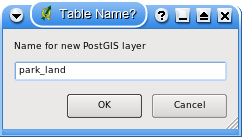
\includegraphics[scale=0.8]{gettablename}
\end{center}
\end{figure}

In line 34 we check to see if the user actually entered anything before 
proceeding.

Next we need to get the field names. For this example we are keeping it very 
simple. Every field will be a varchar(10), meaning we can store up to 10 
characters in it. If we really want to make this plugin useful, we would need 
to provide a way for the user to specify the type. In line 36 we 
prompt the user to enter a comma delimited list of field names. 

\begin{figure}[ht]
\begin{center}
  \caption{Enter field names for new PostGIS table}\label{fig:getfieldname}\smallskip
  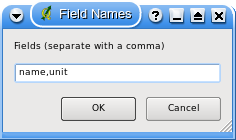
\includegraphics[scale=0.8]{getfieldname}
\end{center}
\end{figure}

We then split this list into its components for use in constructing the SQL 
statement (line 38). 

Line 40 contains the first part of the SQL statement. Note we are 
creating the table with an integer id field that will be the primary key. We 
then iterate through the field list, appending the appropriate code to the 
SQL statement (line 41).

Once we have all the fields added to the SQL statement, we chop off the 
trailing characters we don't want (line 43) and then add 
the closing parenthesis to complete the statement (line 44).

Now we are ready to connect to the database and create the table. To access 
the database, we are using psycopg (\url{http://www.initd.org}). In order 
to connect we need to specify the data source name (DSN) with the name of 
the database, the user, and a password if necessary. If we are running both 
QGIS and PostgreSQL on the same machine we usually don't need to specify a 
password. In this case, the DSN will look something like this:

\begin{center}
  \textsl{dbname=gis\_data user=gsherman}
\end{center}

To get the DSN, we prompt the user with a \textbf{QInputDialog} in line 47.

\begin{figure}[ht]
\begin{center}
  \caption{Enter DSN for connection to PostGIS database}\label{fig:getdsn}\smallskip
  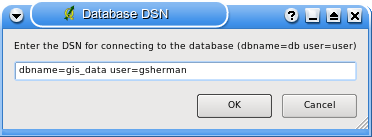
\includegraphics[scale=0.8]{getdsn}
\end{center}
\end{figure}

If the user enters a DSN then we can proceed with the connection to the 
database in line 50. We get a cursor from the connection in 
line 51 and then execute the SQL statement to create the 
table and commit the change in lines 52 through 53. 
This creates the table, but for it to be a valid layer and ready for us to
use it needs a couple more things. 

First it needs a geometry column. We purposely didn't include one
when we created the table so we could use the \textsl{AddGeometryColumn} 
function to create it. This function adds a geometry column to the table 
and then puts an entry in the \textsl{geometry\_columns} table for us. In 
line 55 we specify the table name, the name we want for the 
geometry column, the SRID, feature type, and the dimension of the feature. 

The last thing to do is create a spatial index on the table so we get 
optimum performance when doing spatial searches and displaying the data 
in QGIS. In line 59 we have cobbled together the SQL to create the 
index. The actual statement looks like this:

\begin{verbatim}
create index sidx_park_land on park_land 
   USING GIST(the_geom GIST_GEOMETRY_OPS);
\end{verbatim}

\subsubsection{Issues and Problems}

Our plugin is now complete. Now lets look at some of the things that are 
wrong with it or where we could improve it:

\begin{itemize}
\item We could use an improved GUI, one that lets the user enter all the 
  needed information on one dialog
\item The user can't specify field types
\item There is limited error checking in the dialog
  \begin{itemize}
    \item If you don't enter any fields, the plugin fails
    \item There is no error checking on any of the database operations
  \end{itemize} 
\item There is no feedback from the plugin once it completes
\end{itemize} 

With all the issues, it still serves as a primordial plugin that illustrates 
the process and helps get you started with your own plugin development.

\subsubsection{Adding Feedback}

Let's fix one of the small problems by adding some feedback at the end of 
the process. We'll just add a message box to tell the user that everything 
is done and to check the database to make sure the table was created.

To do this, we just add the following code after line 61:

\begin{verbatim}
# show the user what happened
QMessageBox.information(None, "Results", "Table " + str(table_name[0]) + \
" has been created. Check your database to confirm.")
\end{verbatim}

When the table is created, the user sees this:

\begin{figure}[ht]
\begin{center}
  \caption{Message Box with Plugin results}\label{fig:plugin_results}\smallskip
  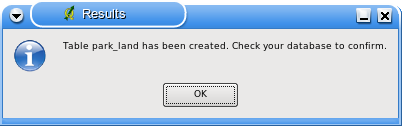
\includegraphics[scale=0.8]{plugin_results}
\end{center}
\end{figure}

\subsubsection{Summary}
Writing a QGIS plugin in Python is pretty easy. Some plugins won't require a
GUI at all. For example, you might write a plugin that returns the map
coordinates for the point you click on the map. Such a plugin wouldn't
require any user input and could use a standard Qt \textbf{QMessageBox}
to display the result. 

You can also write plugins for QGIS in C++, but that's another story. You can 
find tutorials on writing QGIS plugins in both C++ and Python on the QGIS 
blog at:

\begin{center}
  \url{http://blog.qgis.org} 
\end{center}

% vim:tw=76:autoindent
